% $Header: /Users/joseph/Documents/LaTeX/beamer/solutions/generic-talks/generic-ornate-15min-45min.en.tex,v 90e850259b8b 2007/01/28 20:48:30 tantau $

\documentclass{beamer}

% This file is a solution template for:

% - Giving a talk on some subject.
% - The talk is between 15min and 45min long.
% - Style is ornate.



% Copyright 2004 by Till Tantau <tantau@users.sourceforge.net>.
%
% In principle, this file can be redistributed and/or modified under
% the terms of the GNU Public License, version 2.
%
% However, this file is supposed to be a template to be modified
% for your own needs. For this reason, if you use this file as a
% template and not specifically distribute it as part of a another
% package/program, I grant the extra permission to freely copy and
% modify this file as you see fit and even to delete this copyright
% notice. 


\mode<presentation>
{
  \usetheme{Warsaw}
  % or ...

  \setbeamercovered{transparent}
  % or whatever (possibly just delete it)
}


\usepackage[english]{babel}
% or whatever

\usepackage[latin1]{inputenc}
% or whatever

\usepackage{times}
\usepackage[T1]{fontenc}
% Or whatever. Note that the encoding and the font should match. If T1
% does not look nice, try deleting the line with the fontenc.

\graphicspath{{images/}}

\title{Tricolorings of Knots}

\author{Lucas Meyers}
% - Use the \inst{?} command only if the authors have different
%   affiliation.

\institute[Louisiana State University] % (optional, but mostly needed)
{Department of Mathematics\\
Louisiana State University}

\date[Short Occasion] % (optional)
{\today}

\begin{document}

\begin{frame}
  \titlepage
\end{frame}

\section{Tricoloring Knots}

\begin{frame}
  \frametitle{Knot Definition}
  \begin{itemize}
  \item A \textit{Knot} is a simple closed curve in $S^3$ ($\mathbb{R}^3\cup \{\infty\}$)
  \end{itemize}
\end{frame}

\begin{frame}
  \frametitle{Unknot}
  \begin{center}
    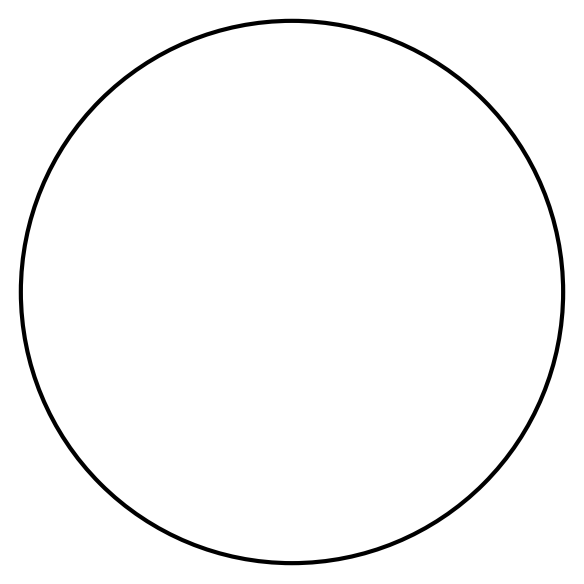
\includegraphics[scale=.4]{unknot}  
  \end{center}
\end{frame}

\begin{frame}
  \frametitle{Trefoil}
  \begin{center}
    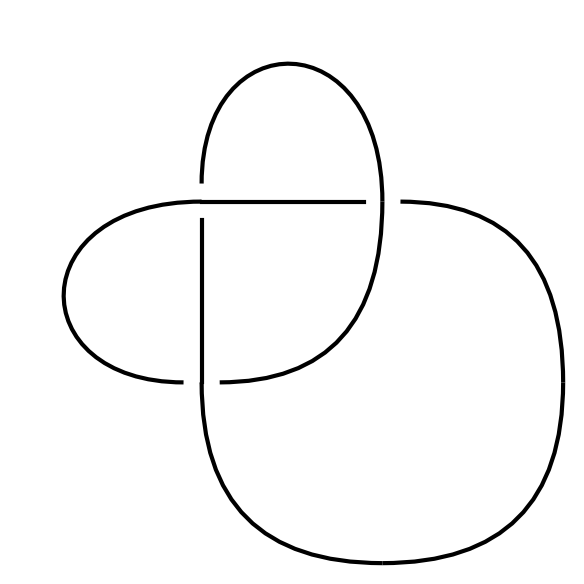
\includegraphics[scale=.4]{trefoil}    
  \end{center}
\end{frame}

\begin{frame}
  \frametitle{Figure-Eight}
  \begin{center}
    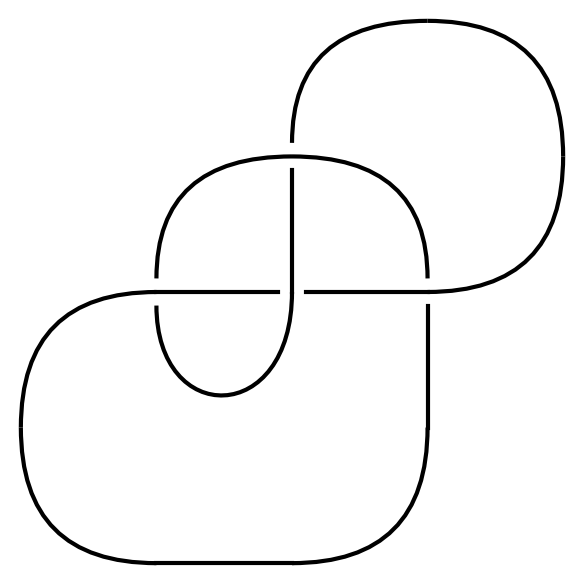
\includegraphics[scale=.4]{figure-eight}
  \end{center}
\end{frame}

\begin{frame}
  \frametitle{Equivalence}
  \begin{itemize}
  \item All knots are homeomorphic to $S^1$.
  \item Two knots $K$ and $J$ are \textit{Ambient Isotopic}
    if there is a homotopy $H:S^3\times[0,1]\rightarrow S^3$ such that
    \begin{itemize}
    \item $H(x,0)$ is the identity on $S^3$
    \item The image $H(K,1)$ is $J$
    \item For each fixed $t\in[0,1]$ the map $H(x,t)$ is a
      homeomorphism.
    \end{itemize}
  \end{itemize}
\end{frame}

\begin{frame}
  \frametitle{Diagrams}
  \begin{itemize}
  \item A \textit{diagram} $D$ of a knot $K$ is a projection of
    $K$ to a plane such that
    \begin{itemize}
    \item We preserve over and under crossing information
    \item Only two points or fewer may be projected to the same
      point
    \item All crossings must be either overcrossings or undercrossings.
      
    \end{itemize}
    \begin{center}
      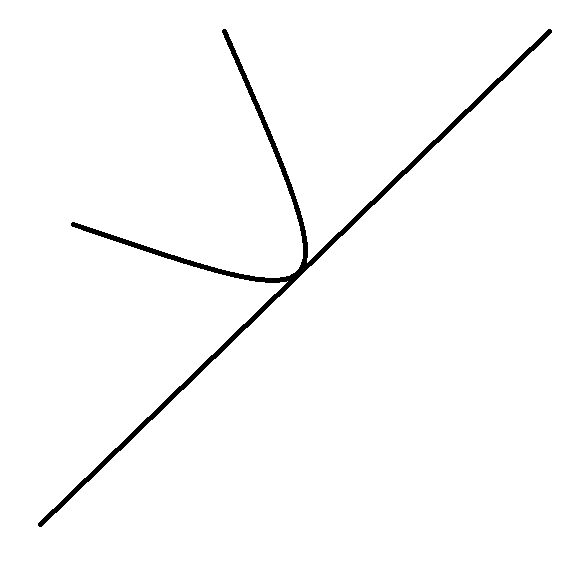
\includegraphics[scale=.2]{bad-crossing}  
    \end{center}
  \end{itemize}
\end{frame}

\begin{frame}
  \frametitle{Reidmeister Moves}
  \begin{itemize}
  \item Diagrams for a knot are not unique.
  \end{itemize}
  \begin{columns}
    \begin{column}{.5\textwidth}
      \begin{center}
        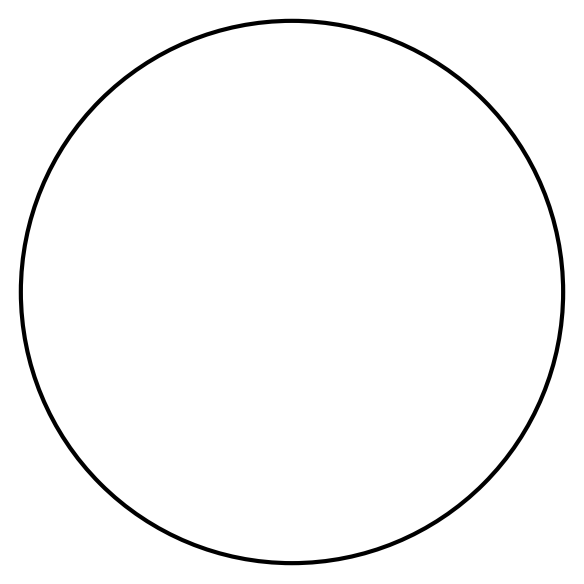
\includegraphics[scale=.3]{unknot}
      \end{center}
    \end{column}
    \begin{column}{.5\textwidth}
      \begin{center}
        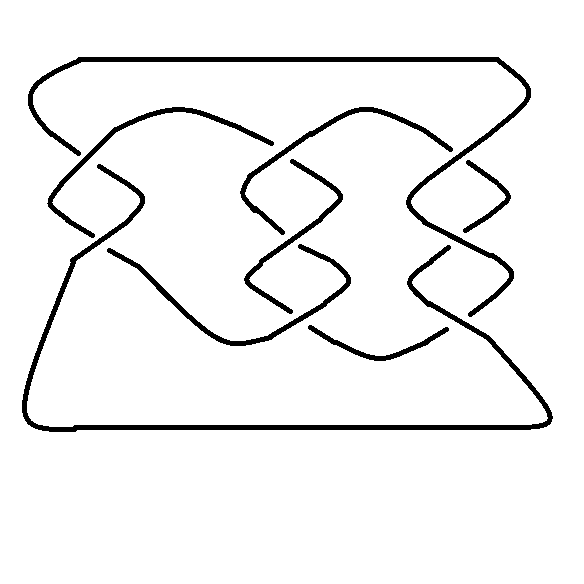
\includegraphics[scale=.3]{ugly-unknot}
      \end{center}
    \end{column}
  \end{columns}
\end{frame}

\begin{frame}
  \frametitle{Reidmeister Moves}
  \begin{itemize}
  \item \textbf{Theorem:} Two knots $K$ and $J$ are ambient isotopic if, and
    only if, their diagrams are related by a finite sequence of Reidmeister moves
    and planar isotopy.
  \end{itemize}
\end{frame}

\begin{frame}
  \frametitle{Type I}
  \begin{center}
    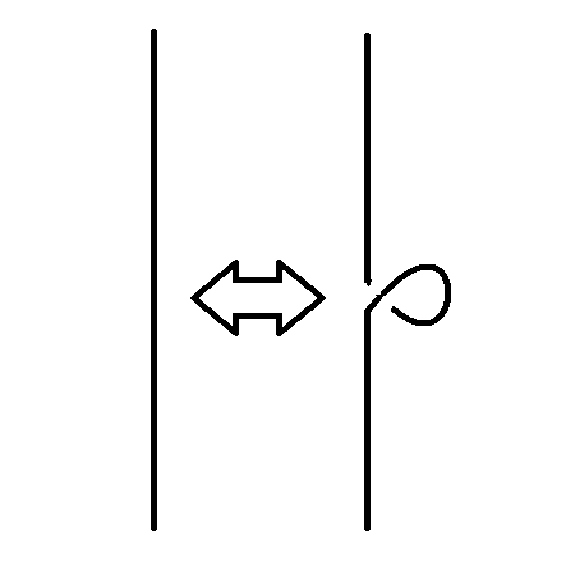
\includegraphics[scale=.4]{t1}
  \end{center}
\end{frame}

\begin{frame}
  \frametitle{Type II}
  \begin{center}
    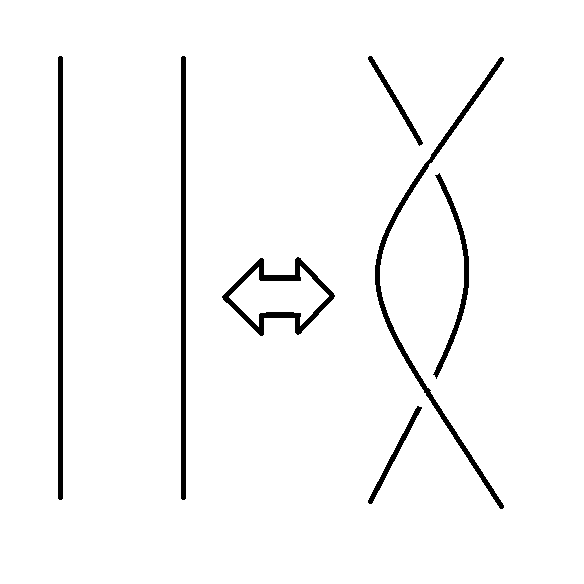
\includegraphics[scale=.4]{t2}
  \end{center}
\end{frame}

\begin{frame}
  \frametitle{Type III}
  \begin{center}
    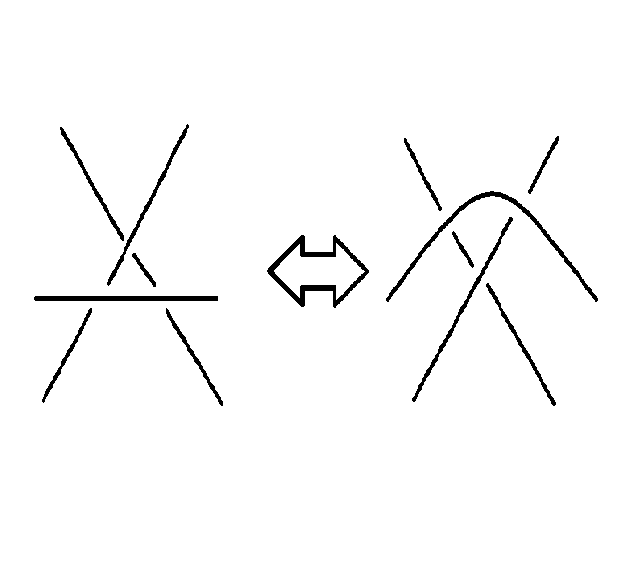
\includegraphics[scale=.6]{t3}
  \end{center}
\end{frame}

\begin{frame}
  \frametitle{Tricoloring}
  \begin{itemize}
  \item A \textit{tricoloring} of a diagram is an assignment
    of one of three colors to each arc such that for all crossings
    \begin{itemize}
    \item Only a single color is present
    \item All three colors are present
    \end{itemize}
  \item A tricoloring is \textit{nontrivial} if at least two colors are used
  \item \textbf{Theorem:} The existence of a non-trivial tricoloring is a knot
    invariant. Such a knot is called tricolorable (or $3$-colorable).
  \end{itemize}
\end{frame}

\begin{frame}
  \frametitle{Type I}
  \begin{center}
    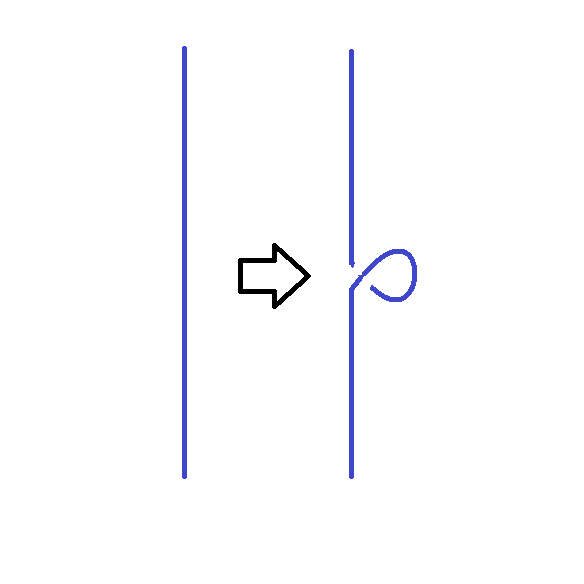
\includegraphics[scale=.4]{t1-c}
  \end{center}
\end{frame}

\begin{frame}
  \frametitle{Type II}
  \begin{center}
    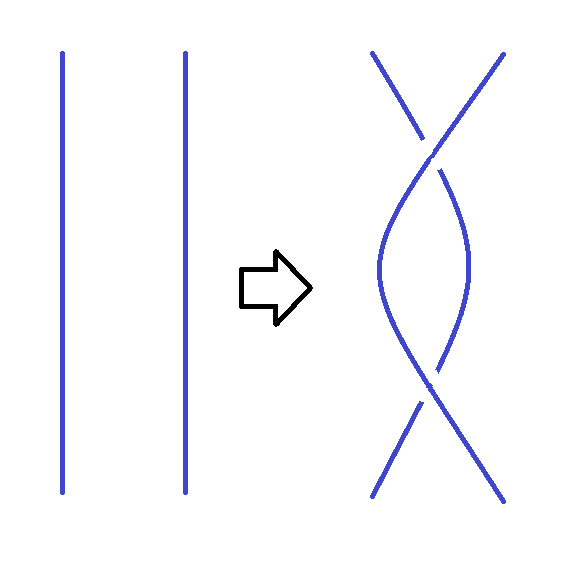
\includegraphics[scale=.4]{t2-c1}
  \end{center}
\end{frame}

\begin{frame}
  \frametitle{Type II}
  \begin{center}
    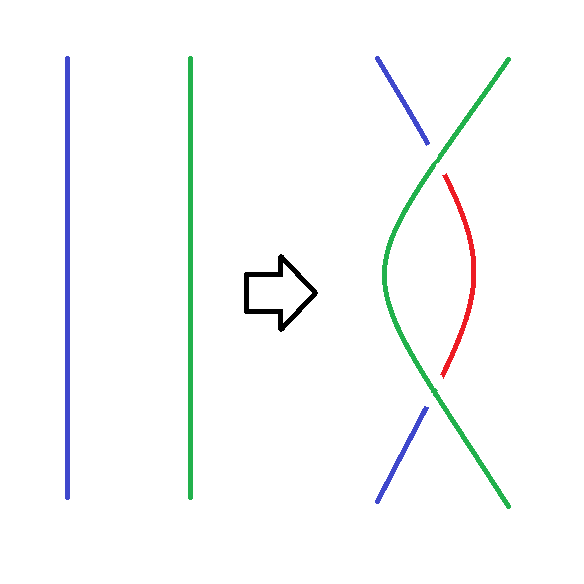
\includegraphics[scale=.4]{t2-c2}
  \end{center}
\end{frame}

\begin{frame}
  \frametitle{Type III}
  \begin{center}
    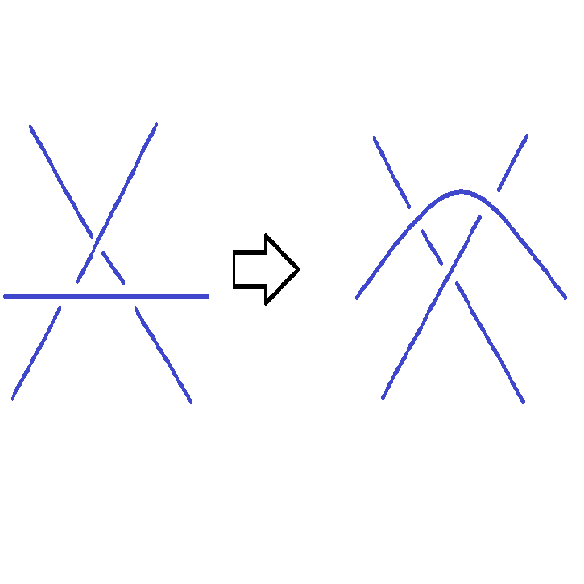
\includegraphics[scale=.6]{t3-c1}
  \end{center}
\end{frame}

\begin{frame}
  \frametitle{Type III}
  \begin{center}
    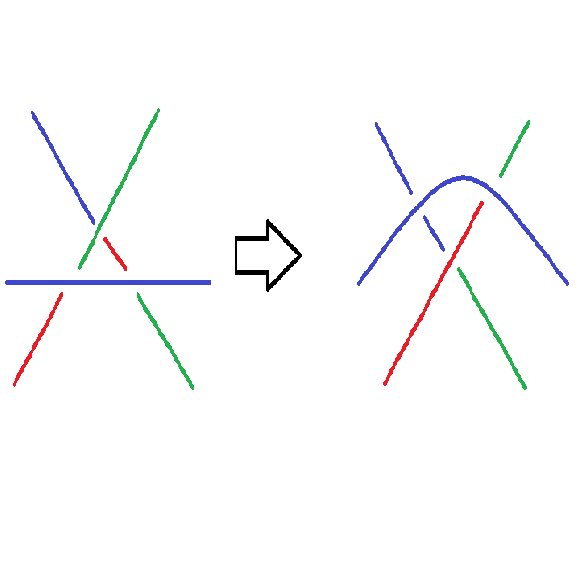
\includegraphics[scale=.6]{t3-c2}
  \end{center}
\end{frame}

\begin{frame}
  \frametitle{Type III}
  \begin{center}
    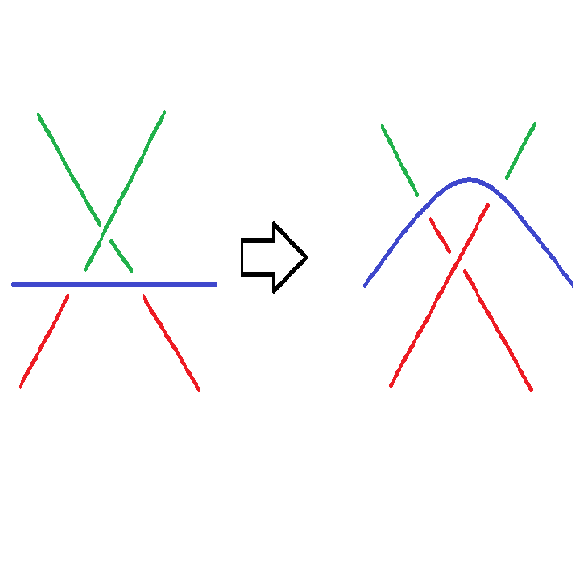
\includegraphics[scale=.6]{t3-c3}
  \end{center}
\end{frame}

\begin{frame}
  \frametitle{Uncolorability of the Unknot}
  \begin{center}
    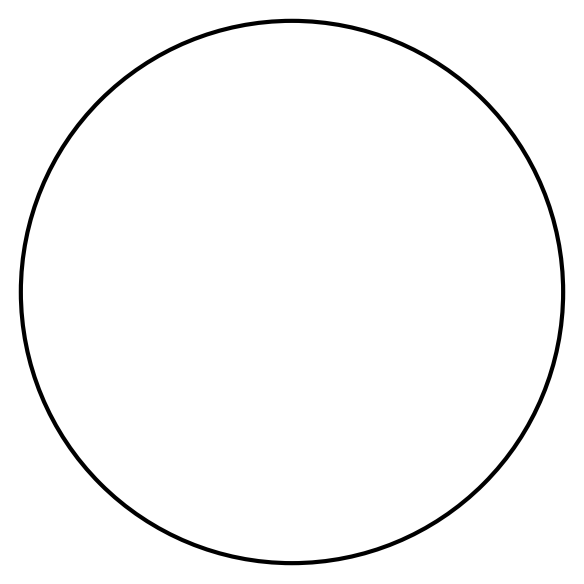
\includegraphics[scale=.4]{unknot}
  \end{center}
\end{frame}

\begin{frame}
  \frametitle{Colorability of the Trefoil}
  \begin{center}
    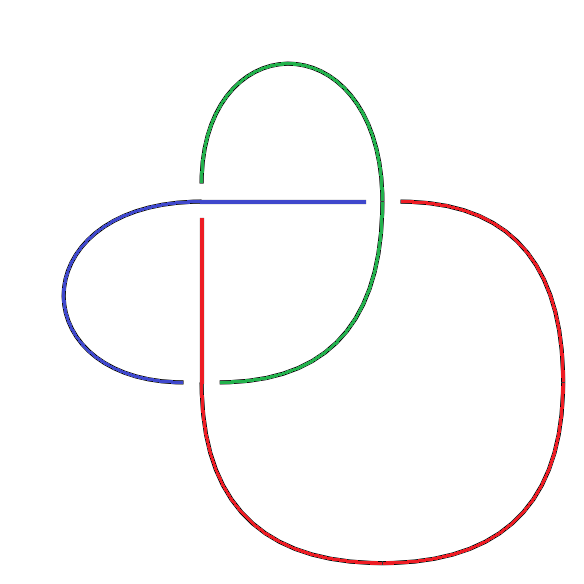
\includegraphics[scale=.4]{trefoil-c}
  \end{center}
\end{frame}

\begin{frame}
  \frametitle{Uncolorability of the Figure-Eight Knot}
  \begin{center}
    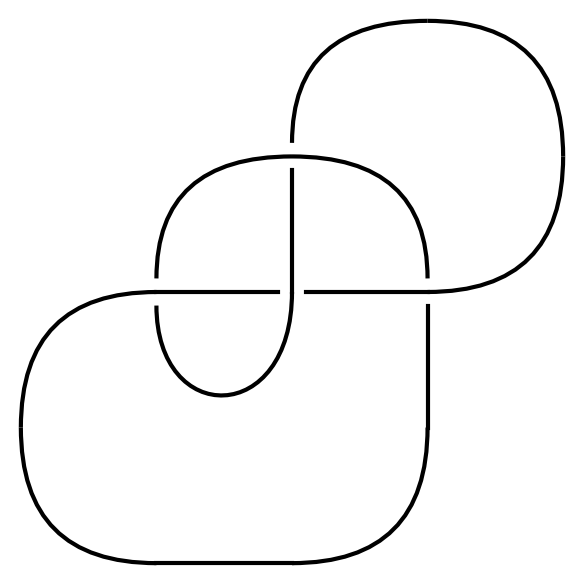
\includegraphics[scale=.4]{figure-eight}
  \end{center}
\end{frame}

\section{The Knot Group}

\begin{frame}
  \frametitle{Knot Group}
  \begin{itemize}
  \item Since all knots are homeomorphic to $S^1$ their
    fundamental groups are isomorphic to $\mathbb{Z}$.
  \item Given a knot $K$, the \textit{knot group} is
    the fundamental group of the knots complement  $\pi_1(S^3\setminus K,*)$
  \end{itemize}
\end{frame}

\begin{frame}
  \frametitle{Knot Group of the Unknot}
  \begin{center}
    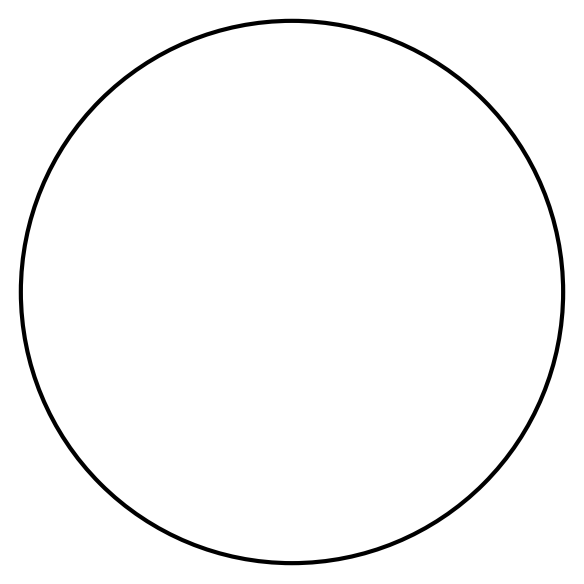
\includegraphics[scale=.3]{unknot}
  \end{center}
  \begin{itemize}
  \item The knot group of the unknot is
    $\pi_1(S^3\setminus K,*)=\mathbb{Z}$ generated by the loop through the
    unknot's.
  \end{itemize}
\end{frame}

\begin{frame}
  \frametitle{Wirtinger Presentation}
  \begin{itemize}
  \item For other knots we use a tool called the \textit{Wirtinger Presentation}.
  \item Let $K$ be a knot and $D$ a diagram for $K$. Choose an orientation of $D$.
    Let $x_1,\ldots, x_n$ denote the arcs of $D$ and, for each crossing, give a
    relation $r_1,\ldots, r_m$ such that $r_i\equiv (x_i x_j x_i^{-1})$ where, when approaching
    $x_k$ is the arc leaving the crossing, the top arc is $x_i$ and the bottom arc entering
    is $x_j$.
  \item Then the knot group of $K$ has presentation
    \[
      \pi_1(S^3\setminus K) \equiv \langle x_1,\ldots, x_n| r_1,\ldots r_m\rangle
    \]
  \end{itemize}
\end{frame}

\begin{frame}
  \frametitle{Knot Group of the Trefoil}
  \begin{center}
    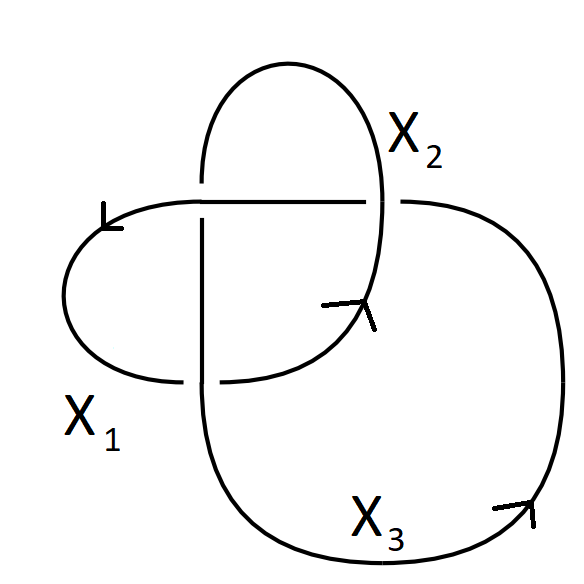
\includegraphics[scale=.25]{annotated-trefoil}
  \end{center}
  \begin{itemize}
  \item From this diagram the knot group of the trefoil is 
    \[
      \langle x_1,x_2,x_3|x_1x_2x_1^{-1}=x_3,x_3x_1x_3^{-1}=x_2,x_2x_3x_2^{-1}=x_1\rangle
    \]
  \item Which simplifies to $\langle x_1,x_2|x_1 x_2 x_1= x_2 x_1 x_2\rangle$
  \end{itemize}
\end{frame}

\begin{frame}
  \frametitle{Fox 3-Colorings}
  \begin{itemize}
  \item A \textit{Fox $3$-coloring} is a homomorphism $\rho$ from
    the knot group the symmetry group $D_6$ of an equilateral
    triangle.
  \item A Fox $3$-coloring is nontrivial if $\rho$ is surjective.
  \end{itemize}
\end{frame}

\begin{frame}
  \frametitle{Fox 3-Colorings of the Unknot and Trefoil}
  \begin{itemize}
  \item There is no nontrivial Fox $3$-coloring of the unknot as
    $D_6$ has two generators and the knot group of the unknot, $\mathbb{Z}$,
    only has one.
  \item We can give a nontrivial Fox $3$-coloring of the trefoil,
    $\langle x_1,x_2|x_1 x_2 x_1= x_2 x_1 x_2\rangle$, using the presentation of $D_6$ as
    \[
      \langle r,s| r^3=s^2=1, srsr=1\rangle
    \]
    by mapping $x_1$ to $r$ and $x_2$ to $s$ or vice versa.
  \item This gives us two nontrivial Fox $3$-colorings of the trefoil.
   \end{itemize}
\end{frame}

\begin{frame}
  \frametitle{Equivalence of Tricoloring and Fox 3-Coloring}
  \begin{itemize}
  \item \textbf{Theorem:} A Knot $K$ has a $3$-coloring if, and only if,
    there is a Fox $3$-coloring of $K$.
  \end{itemize}
\end{frame}

\section{Consequences}

\begin{frame}
  \frametitle{Consequences}
  \begin{itemize}
  \item Since for any two groups $G$ and $H$ the homomorphisms
    $\hom(G,H)$ form a group this implies that colorings of knots
    also form a group.
  \item Unlike with tricolorability it more obvious how to extend
    Fox $3$-colorings to an arbitrary number of colors.
    \begin{itemize}
    \item A \textit{Fox $n$-coloring} of a knot $K$ is a homomorphism from
      the knot group of $K$ to $D_{2n}$.
    \end{itemize}
  \item Given any group $G$ we can define a \textit{Fox $G$-coloring}
    as a homomorphism from the knot group of $K$ to the group $G$.
    \begin{itemize}
    \item If $G$ is a finite group then searching for nontrivial $G$-colorings
      is very fast to compute.
    \item This can be done by sending generators to generators and checking
      that the relations hold.
    \end{itemize}
  \end{itemize}
\end{frame}

\begin{frame}
  \frametitle{Extending Tricolorability}
  \begin{itemize}
  \item We can also use the fact that Fox $3$-colorings and tricolorability
    are equivalent to guide us in extending the notion of $n$-colorings
    to diagrams as well.
  \item Instead of assigning colors to each arc we use elements of $\mathbb{Z}_n$.
  \item Then a diagram has a nontrivial coloring if at least two numbers are used
    and for each crossing, if we label the overcrossing arc $x$ and the two
    undercrossing arcs as $y$ and $z$, the following equation is satisfied
    \[
      2x-y-z \equiv 0 \mod n
    \]
  \end{itemize}
\end{frame}

\begin{frame}
  \frametitle{5-Coloring of the Figure-Eight Knot}
  \begin{itemize}
  \item Recall that the figure-eight knot was not $3$-colorable.
    However it is $5$-colorable.
  \end{itemize}
  \begin{center}
    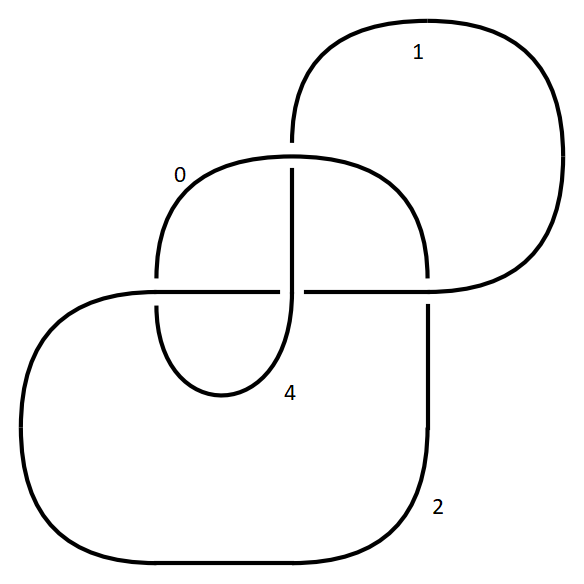
\includegraphics[scale=.4]{figure-eight-c}
  \end{center}
\end{frame}

\end{document}


